\documentclass[11pt,a4paper]{article}
\usepackage[T1]{fontenc}
\usepackage[utf8]{inputenc}
\usepackage{mathpazo}
\usepackage{courier}
\usepackage[margin=2.5cm]{geometry}
\usepackage{graphicx}
\usepackage{booktabs}
\usepackage{float}
\usepackage{array}
\usepackage{microtype}
\usepackage[font=small,labelfont=bf]{caption}
\usepackage{enumitem}
\usepackage[hidelinks]{hyperref}
\usepackage{url}
\setlength{\parskip}{0.5em}
\setlength{\parindent}{0pt}
\linespread{1.05}
\setlist{itemsep=0.2em,topsep=0.3em}
\newcommand{\ra}{$\rightarrow$}
\hypersetup{pdftitle={Is It the Encoder or the Probe? Acquisition-Artifact Robustness of Pathology Foundation Models},pdfauthor={Dinakar Pathakota}}

\title{\textbf{Is It the Encoder or the Probe?\\ Acquisition-Artifact Robustness of Pathology Foundation Models}}
\author{Dinakar Pathakota\\[0.3em]
\small Independent Researcher, Hyderabad, India\\
\small \texttt{dinakar.pathakota@gmail.com}}
\date{5 October 2026\\[0.3em]\small Technical report, version 1}

\begin{document}
\maketitle

\begin{abstract}
\noindent Pathology foundation models are usually judged for robustness by training a linear probe on clean images and testing it on degraded ones. We ask how much of the measured brittleness comes from the frozen encoder and how much from the probe. We evaluate three pathology encoders (Phikon, Phikon-v2, Kaiko ViT-B/16) and one natural-image encoder (DINOv2-L) on NCT-CRC-HE and PatchCamelyon under controlled blur, JPEG compression and stain shift. A probe trained on a mix of clean and degraded embeddings recovers most of the accuracy lost to compression: for Phikon-v2 at JPEG quality 15 on NCT-CRC-HE, balanced accuracy rises from 76.3\% to 92.5\%, and at quality 10, which the probe never saw, from 49.1\% to 88.1\%. The effect holds for all four encoders, both datasets, two regularisation strengths and five seeds, and changes clean accuracy by between $-1.2$ and $+2.4$ points. Model rankings depend on the probe: with a clean-trained probe DINOv2-L beats all three pathology encoders under heavy compression, and with the mixed probe the pathology encoders match or beat it. Blur at low magnification is only partly recoverable, training on one artifact does not transfer reliably to another, and embedding drift does not predict accuracy loss across encoders. We recommend that robustness benchmarks report probe settings and include a degradation-aware probe as a baseline. Code and results: \url{https://github.com/dinakar0745/encoder-or-probe}.
\end{abstract}

\section{Introduction}

Foundation models for histopathology are now routinely used as frozen feature extractors, with a small classifier trained on top for each task. Whether these models stay accurate when image quality drops matters in practice: whole-slide scanners produce out-of-focus regions, archives are compressed to save storage, and staining varies between laboratories.

Recent benchmarks measure this robustness with a common protocol. A linear probe is trained on clean images, and the same probe is then tested on perturbed images, for example blurred, compressed or stain-shifted ones (Yajnik et al., 2026). The resulting accuracy drop is reported as a property of the encoder, and encoders are ranked by it. Two things are usually left unreported: how the probe was regularised, and what happens if the probe has seen degraded images during training.

This leaves an open question. A frozen encoder may preserve the information needed to classify a degraded image while moving its embedding to a region the clean-trained probe has never seen. In that case the failure belongs to the probe, and a different probe would fix it without touching the encoder. If the information is destroyed, no probe can recover it.

We test this directly. For four encoders and two datasets, we compare a clean-trained probe with a probe trained on a mix of clean and degraded embeddings, holding the training-set size fixed, at two regularisation strengths and over five seeds. Our contributions are:

\begin{enumerate}
\item \textbf{Much of the measured brittleness belongs to the probe.} The mixed probe recovers most of the accuracy lost to JPEG compression and stain shift for every encoder, including at degradation levels it was not trained on, at a cost of about one point or less on clean images.
\item \textbf{Rankings depend on the probe.} Under the clean probe, natural-image DINOv2-L is more robust to heavy compression than all three pathology encoders. Under the mixed probe the gap closes or reverses, and the three pathology encoders become nearly indistinguishable.
\item \textbf{We identify what is not recoverable.} Blur at low magnification removes information that no linear probe recovers, and training on one artifact does not transfer reliably to another.
\item \textbf{Two common proxies are unreliable.} Under JPEG compression on PatchCamelyon, probe regularisation changes measured robustness by up to 25 points for one encoder and under 6 points for another, and embedding drift does not predict accuracy loss across encoders.
\end{enumerate}

We do not propose the mixed probe as a new method. It is a simple baseline, and its value here is what it shows about how robustness is measured.

\section{Related work}

\textbf{Robustness benchmarks for pathology encoders.} Yajnik et al.\ (2026) evaluate 12 pathology foundation models on four patch-level tasks, each reduced to binary classification, under eleven pixel-level, stain and geometric perturbations. A single linear layer is trained on clean data, each perturbation is optimised within a budget to maximise the loss, and robustness is summarised as ROC-AUC averaged over the budget sweep. They find that compression, noise and brightness changes are the most damaging, that blur and other geometric changes are tolerated best, and that robustness correlates weakly with model size. Bareja et al.\ (2026) compare 32 general and pathology-specific models on 41 tasks with linear probing but do not test image corruptions. Neither reports probe hyperparameters or trains a probe on perturbed data. Our study is narrower in models and tasks and adds the probe as an experimental variable. Our perturbations have fixed severity rather than being worst-case within a budget, and we report balanced accuracy, so our numbers are not directly comparable with theirs.

\textbf{Compression and representation drift.} Hasan et al.\ (2026) measure embedding drift under JPEG2000 compression for UNI, Phikon-v2 and DINOv2 on 4,000 TCGA-BRCA tiles from two slides, and find that the pathology encoders drift far more than DINOv2 at the same image fidelity. They measure drift and nearest-neighbour stability, not downstream accuracy. Using baseline JPEG rather than JPEG2000, we find a gap in the same direction in accuracy under a clean probe, show that it closes under a mixed probe, and show that drift magnitude does not predict accuracy loss across encoders.

\textbf{Batch effects and encoder-level fixes.} A separate line of work measures sensitivity to the medical centre, scanner and staining protocol on frozen encoders (de Jong et al., 2025; Grisi et al., 2026) and reduces it by fine-tuning the encoder (Filiot et al., 2026). We study acquisition artifacts and leave the encoder frozen.

\textbf{Augmentation on frozen features.} B\"ar et al.\ (2024) augment frozen features and train a lightweight head for few-shot classification on natural images. Our mixed probe is related but degrades the image before the encoder, and we use it to study robustness, which they do not evaluate.

\textbf{Transfer between corruptions.} Geirhos et al.\ (2018) show that networks trained on one distortion do not generalise to others. We observe the same for linear probes on frozen pathology encoders.

\textbf{Dataset caveats.} Ignatov and Malivenko (2024) report class-dependent JPEG artifacts and colour bias in NCT-CRC-HE. We therefore replicate every result on PatchCamelyon.

\section{Method}

\subsection{Encoders}

\begin{table}[h]\centering\small
\caption{Encoders. All are frozen and used with the preprocessing published with their weights.}
\label{tab:encoders}
\begin{tabular}{@{}l l p{4.6cm} l p{3.1cm}@{}}
\toprule
Encoder & Architecture & Pretraining & Embedding & Preprocessing\\
\midrule
Phikon & ViT-B/16 & iBOT, 40M tiles from TCGA & 768, CLS & resize to 224\\
Phikon-v2 & ViT-L/16 & DINOv2, 456M tiles from 58k slides (TCGA, CPTAC, GTEx and others) & 1024, CLS & resize to 224, centre-crop 224\\
Kaiko B/16 & ViT-B/16 & DINO, 29k TCGA slides & 768, CLS & resize to 224, centre-crop 224\\
DINOv2-L & ViT-L/14 & DINOv2, natural images & 1024, CLS & resize to 256, centre-crop 224\\
\bottomrule
\end{tabular}
\end{table}

Table~\ref{tab:encoders} lists the encoders (Filiot et al., 2023; Filiot et al., 2024; Aben et al., 2024; Oquab et al., 2023). Phikon-v2 and DINOv2-L share an architecture family and training method and differ in training data, which makes them the closest available pair for isolating the effect of pathology pretraining.

\textbf{Pretraining overlap.} No evaluation slide appears in the published pretraining data of any encoder. Phikon and the Kaiko encoder were pretrained on TCGA only. The Phikon-v2 pretraining set is itemised in Extended Table 6 of Filiot et al.\ (2024): 132 public and 4 private cohorts, 58,359 slides. Neither Camelyon16 nor the NCT-CRC-HE source slides are listed, and that paper uses Camelyon16 as an external test set. The tissue types are represented, however: all three pathology encoders saw TCGA colorectal slides, and the Phikon-v2 list includes a 130-slide breast metastasis cohort from another centre. The contents of the four private cohorts are not public.

\subsection{Datasets}

\textbf{NCT-CRC-HE.} Nine tissue classes of colorectal histology in $224 \times 224$ pixel patches at 0.5 microns per pixel, colour-normalised with Macenko's method (Kather et al., 2018). We train on 9,000 images (1,000 per class) sampled from NCT-CRC-HE-100K and test on all 7,180 images of CRC-VAL-HE-7K, which comes from 50 patients with no overlap with the training set.

\textbf{PatchCamelyon.} Binary detection of metastatic tissue in lymph node sections from Camelyon16 (Ehteshami Bejnordi et al., 2017), in $96 \times 96$ pixel patches at 10x magnification; a patch is positive if its central $32 \times 32$ region contains tumour (Veeling et al., 2018). We train on 9,000 images (4,500 per class) sampled from the validation split and test on 6,000 images (3,000 per class) sampled from the test split.

\subsection{Degradations}

Each degradation is applied to the image at its native resolution, before the encoder's own preprocessing.

\begin{itemize}
\item \textbf{Blur:} Gaussian blur with $\sigma$ of 0.5, 1, 2, 3, 3.5, 4, 5 and 6 pixels.
\item \textbf{Compression:} JPEG at quality 70, 50, 30, 25, 20, 15, 10 and 5.
\item \textbf{Stain shift:} the image is converted to haematoxylin-eosin-DAB space, the haematoxylin channel is multiplied by $(1+\alpha)$ and the eosin channel by $(1-\alpha)$, for $\alpha$ of 0.1 to 0.5.
\end{itemize}

\subsection{Probes}

Every probe is an L2-regularised logistic regression on standardised embeddings (scikit-learn, L-BFGS, at most 2,000 iterations). We report two regularisation strengths, $C = 1$ (default) and $C = 0.001$ (strong).

\begin{itemize}
\item \textbf{Clean probe:} trained on clean embeddings only. This is the standard protocol.
\item \textbf{Mixed probe:} each training image is represented by one embedding drawn at random from its clean version and five degraded versions (blur $\sigma$ 2 and 4, JPEG quality 30 and 15, stain $\alpha$ 0.3). The training set therefore has the same size as for the clean probe.
\item \textbf{Single-artifact probes:} as the mixed probe, but drawing only from the clean version and the degraded versions of one artifact type.
\end{itemize}

Each probe is trained five times. Each seed uses a different random 80\% of the training images and a different random draw of versions. We report the mean and standard deviation of balanced accuracy on the test set.

\subsection{Drift and failure analysis}

For each degraded test image we compute the cosine distance between its embedding and the embedding of its clean version. We relate this drift to the accuracy drop of the clean probe, and we measure how well per-image drift ranks the images whose prediction changes (AUROC). We also report recall per class.

\subsection{Software}

Embeddings were extracted on one NVIDIA RTX 3050 (4 GB) with PyTorch 2.11.0 (CUDA 12.8) and stored as 16-bit floats. Phikon, Phikon-v2 and DINOv2-L were loaded with transformers 5.18.0; the Kaiko encoder was loaded with timm 1.0.30 and torchvision 0.26.0 in a separate environment. Degradations used Pillow 12.3.0 and scikit-image 0.26.0 in both environments. Probes used scikit-learn 1.9.1 with NumPy 2.5.3 and SciPy 1.18.1. Both environments ran Python 3.14.8 on Windows.

\section{Results}

All figures are balanced accuracy in \%, mean of five seeds. Unless stated, results use $C = 1$. For the clean and mixed probes, standard deviations over seeds are below 2 points in 97\% of cells on NCT-CRC-HE (maximum 4.3) and in 86\% of cells on PatchCamelyon (maximum 5.1). The single-artifact probes vary more between seeds, by up to 11.4 points. Full tables for the clean and mixed probes are in the appendix (Tables~\ref{tab:app1} to~\ref{tab:app4}); the single-artifact probes, drift and per-class recall are in the code repository.

\subsection{The clean probe degrades sharply}

Under the standard protocol every encoder has a cliff. On NCT-CRC-HE the three pathology encoders lose at most 4 points under JPEG down to quality 30 (91.6 to 93.3, against 93.8 to 95.6 clean) and then fall to 72.8 (Phikon), 49.1 (Phikon-v2) and 53.3 (Kaiko) at quality 10. Under blur they fall to 67.4, 82.6 and 59.0 at $\sigma = 4$. DINOv2-L starts lower (88.0 clean), degrades slowly under JPEG (79.4 at quality 10) and quickly under blur (54.5 at $\sigma = 4$).

PatchCamelyon breaks much earlier. Its patches are 96 pixels at lower magnification and are enlarged before the encoder, so the same $\sigma$ or quality level is a larger perturbation. At JPEG quality 30 the pathology encoders reach 54.4 to 63.2, against about 80 clean, and at blur $\sigma = 2$ they reach 52.8 to 62.8, where 50 is chance.

\subsection{A mixed probe recovers most of the loss}

Table~\ref{tab:main} and Figure~\ref{fig:grid} compare the clean probe with the mixed probe. On NCT-CRC-HE the mixed probe brings every pathology encoder back to about 92 at JPEG quality 15 and about 88 at quality 10, a level it never saw in training. Blur at $\sigma = 4$ recovers to 90.7 to 92.5. On PatchCamelyon, JPEG quality 15 recovers from chance to 75.8 to 79.5 at the default setting and to 81.6 to 84.7 at the strong setting. Across all 16 combinations of encoder, dataset and regularisation, the mixed probe changes clean accuracy by between $-1.2$ and $+2.4$ points.

\begin{table}[h]\centering\small
\caption{Clean probe \ra{} mixed probe, balanced accuracy in \%, $C = 1$. ``Unseen'' marks conditions the mixed probe was not trained on.}
\label{tab:main}
\begin{tabular}{@{}lcccc@{}}
\toprule
Condition & Phikon & Phikon-v2 & Kaiko B/16 & DINOv2-L\\
\midrule
NCT, clean & 93.8 \ra{} 93.6 & 94.1 \ra{} 94.6 & 95.6 \ra{} 95.0 & 88.0 \ra{} 88.3\\
NCT, JPEG Q15 & 84.0 \ra{} 92.0 & 76.3 \ra{} 92.5 & 74.8 \ra{} 92.0 & 83.1 \ra{} 87.4\\
NCT, JPEG Q10 (unseen) & 72.8 \ra{} 89.2 & 49.1 \ra{} 88.1 & 53.3 \ra{} 87.9 & 79.4 \ra{} 84.4\\
NCT, blur $\sigma$ 3 (unseen) & 87.4 \ra{} 92.4 & 91.8 \ra{} 93.5 & 86.9 \ra{} 93.0 & 66.3 \ra{} 85.8\\
NCT, blur $\sigma$ 4 & 67.4 \ra{} 91.4 & 82.6 \ra{} 92.5 & 59.0 \ra{} 90.7 & 54.5 \ra{} 81.6\\
NCT, stain $\alpha$ 0.5 (unseen) & 86.9 \ra{} 90.6 & 86.1 \ra{} 91.9 & 92.2 \ra{} 93.6 & 86.9 \ra{} 88.0\\
\addlinespace
PCam, clean & 81.3 \ra{} 82.9 & 80.5 \ra{} 82.3 & 80.2 \ra{} 82.5 & 80.2 \ra{} 82.6\\
PCam, JPEG Q15 & 53.7 \ra{} 79.5 & 49.9 \ra{} 75.8 & 50.1 \ra{} 79.2 & 66.8 \ra{} 77.5\\
PCam, blur $\sigma$ 4 & 51.3 \ra{} 70.5 & 55.0 \ra{} 67.2 & 50.3 \ra{} 71.4 & 58.9 \ra{} 67.9\\
\bottomrule
\end{tabular}
\end{table}

\begin{figure}[t]\centering
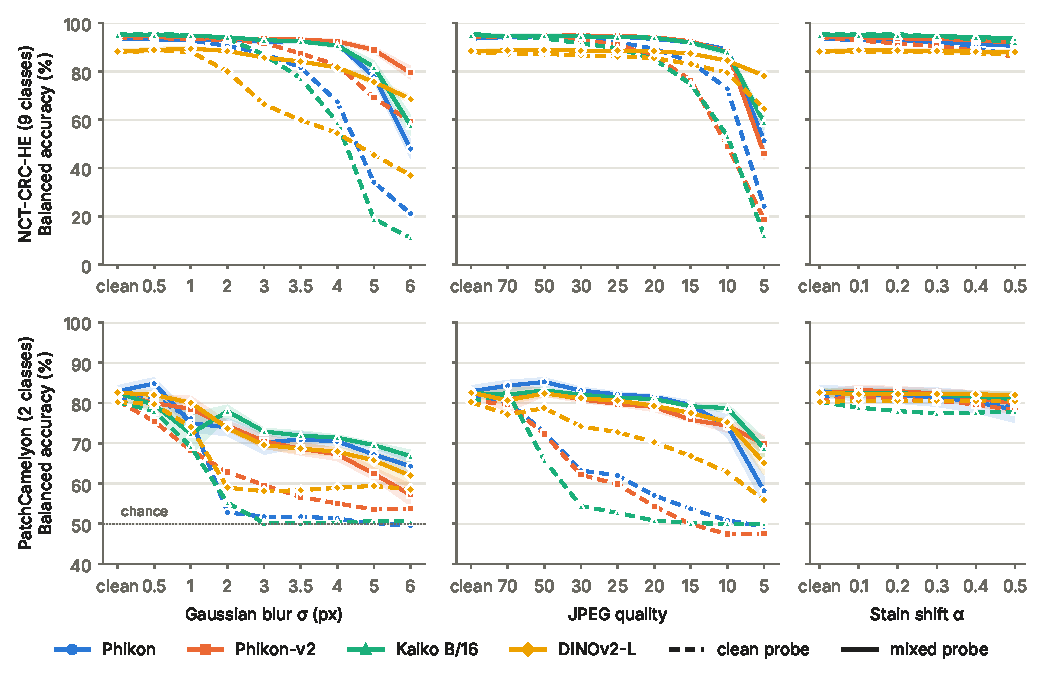
\includegraphics[width=\linewidth]{fig2_recovery_grid.pdf}
\caption{Balanced accuracy under blur, JPEG compression and stain shift on NCT-CRC-HE (top) and PatchCamelyon (bottom) at $C = 1$. Dashed lines are the clean probe and solid lines the mixed probe. Shaded bands show one standard deviation over five seeds. The dotted line marks chance on PatchCamelyon.}
\label{fig:grid}
\end{figure}

The accuracy lost to compression and stain shift was therefore not lost in the encoder. The embeddings still separate the classes; the clean-trained probe reads them along the wrong direction.

\subsection{Model rankings depend on the probe}

Under the clean probe at JPEG quality 10 on NCT-CRC-HE, DINOv2-L (79.4) is more accurate than all three pathology encoders (72.8, 49.1, 53.3), although it is 6 to 8 points worse on clean images (Figure~\ref{fig:flip}). Under the mixed probe all three pathology encoders (89.2, 88.1, 87.9) are ahead of it (84.4). At the strong regularisation setting the gap closes without fully reversing: under the clean probe DINOv2-L leads by 7 to 37 points, and under the mixed probe Phikon is ahead (89.1) while Phikon-v2 (87.1), Kaiko (86.1) and DINOv2-L (86.6) are within a point of each other.

The mixed probe also removes most differences between the pathology encoders. Under the clean probe they span 24 points at blur $\sigma = 4$ (59.0 to 82.6) and 24 points at JPEG quality 10. Under the mixed probe they are within 2 points of each other in both conditions.

\begin{figure}[t]\centering
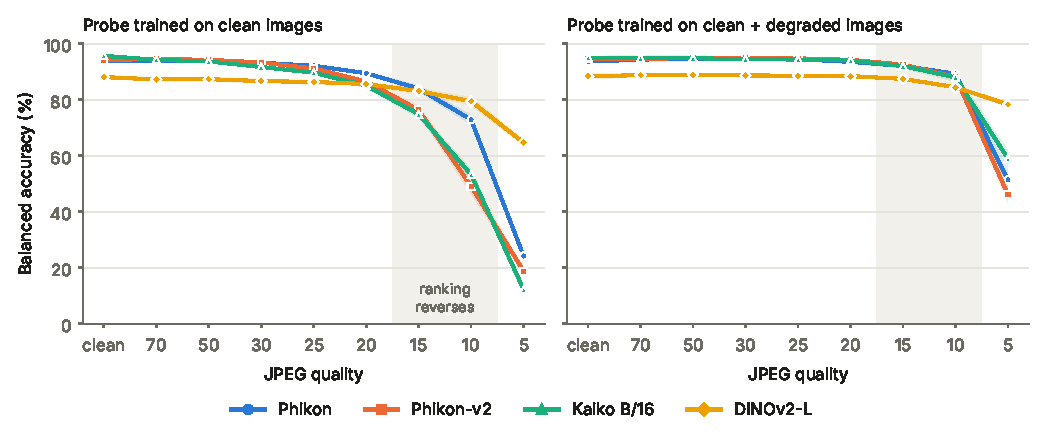
\includegraphics[width=\linewidth]{fig1_ranking_flip.pdf}
\caption{Balanced accuracy under JPEG compression on NCT-CRC-HE at $C = 1$, with a probe trained on clean images (left) and the mixed probe (right). In the shaded range, DINOv2-L leads the pathology encoders under the clean probe and trails them under the mixed probe. Shaded bands around the lines show one standard deviation over five seeds.}
\label{fig:flip}
\end{figure}

\subsection{Regularisation is a model-dependent lever}

Probe regularisation changes measured robustness with no change to the training data (Figure~\ref{fig:reg}). On PatchCamelyon at JPEG quality 30, moving from $C = 1$ to $C = 0.001$ raises the clean probe from 63.2 to 85.0 for Phikon and from 62.1 to 74.8 for Phikon-v2, but only from 54.4 to 57.6 for Kaiko. Clean accuracy improves for all three (to 91.2, 86.7 and 88.3). On NCT-CRC-HE the effect is at most 9 points. A benchmark that fixes one unreported value of $C$ can therefore favour one encoder over another.

\begin{figure}[t]\centering
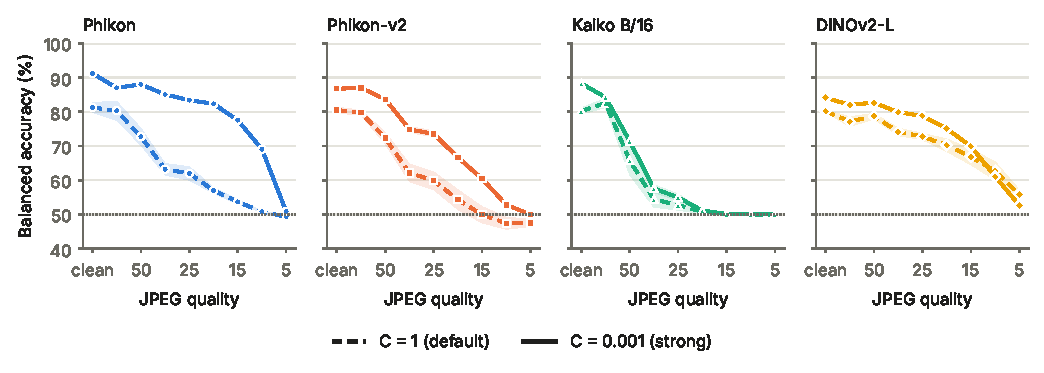
\includegraphics[width=\linewidth]{fig3_regularisation.pdf}
\caption{Clean probe on PatchCamelyon under JPEG compression at two regularisation strengths. Stronger regularisation raises accuracy under compression substantially for Phikon and Phikon-v2 and very little for Kaiko B/16. Shaded bands show one standard deviation over five seeds; the dotted line marks chance.}
\label{fig:reg}
\end{figure}

\subsection{What the mixed probe does not fix}

\textbf{Blur at low magnification.} On PatchCamelyon the mixed probe reaches 67.2 to 71.4 at blur $\sigma = 4$, against about 80 clean. At the strong setting it reaches 67.4 to 72.7 against 84 to 91 clean. This loss is in the image, not the probe.

\textbf{Very heavy compression.} At JPEG quality 5 on NCT-CRC-HE the mixed probe reaches only 46.1 to 58.9 for the pathology encoders, against 78.2 for DINOv2-L.

\textbf{Transfer between artifacts.} A probe trained with blur changes accuracy at JPEG quality 15 by between $-7.0$ and $+16.8$ points across the 16 combinations, relative to the clean probe. A probe trained with JPEG changes accuracy at blur $\sigma = 4$ by between $-5.1$ and $+14.2$ points. The sign is not predictable from the encoder, the dataset or the regularisation strength.

\subsection{Drift and failure direction}

\textbf{Drift does not predict accuracy loss across encoders.} On NCT-CRC-HE at blur $\sigma = 3$, DINOv2-L embeddings drift by 0.18 and accuracy falls 21.7 points, while Phikon-v2 embeddings drift by 0.53 and accuracy falls 2.3 points. Within one encoder, JPEG at quality 70 moves Phikon-v2 embeddings by 0.45 with no accuracy loss, and stain shift at $\alpha = 0.5$ moves them by 0.19 with an 8-point loss. Per-image drift is a weak flag for changed predictions at mild degradation levels (AUROC 0.33 to 0.86, and 0.40 to 0.63 for DINOv2-L).

\textbf{Failures are mostly missed tumours.} On PatchCamelyon at blur $\sigma = 3$, Phikon, Kaiko and DINOv2-L assign almost every image to the normal class at both regularisation settings (tumour recall 0\% to 22\%). Phikon-v2 is the exception: at $C = 1$ it over-predicts tumour (normal recall 41\%), and at $C = 0.001$ it under-predicts it (tumour recall 37\%). On NCT-CRC-HE at blur $\sigma = 4$, tumour recall falls to 27\% for Phikon, 56\% for Kaiko and 19\% for DINOv2-L, from 99\%, 98\% and 88\% on clean images.

\section{Discussion}

\textbf{What benchmarks should report.} A robustness number from a clean-trained linear probe measures the encoder and the probe together. We suggest three additions to the standard protocol: state the probe's regularisation and how it was chosen; report results at more than one regularisation strength; and include a probe trained on degraded examples, so that recoverable and unrecoverable losses can be told apart.

\textbf{What this means for a laboratory.} If a deployment expects compressed or stain-shifted images, a new encoder is not needed. Adding degraded examples when the task head is trained recovers most of the loss at almost no cost. This has to be done for the artifacts actually expected, because training on one does not reliably help with another. Blur at low magnification is different: it removes information, and the remedy is at acquisition.

\textbf{Pathology pretraining and the compression-blur trade-off.} Under the clean probe, the pathology encoders are more sensitive to compression and less sensitive to blur than DINOv2-L. One possible reason is that web images are heavily compressed while scanner images are not, and that slides vary naturally in focus. We did not test this explanation.

\textbf{Blur compared with earlier benchmarks.} Yajnik et al.\ (2026) report blur among the best-tolerated perturbations, while we see large losses under the clean probe at $\sigma = 4$ on NCT-CRC-HE and from $\sigma = 2$ on PatchCamelyon. The two studies differ in severity range, in task definition and in metric, and we did not test which of these accounts for the difference.

\textbf{Drift as a proxy.} Embedding drift is attractive because it needs no labels, but our results caution against comparing encoders by it. An encoder whose embeddings barely move can lose more accuracy than one whose embeddings move a great deal.

\section{Limitations}

\begin{itemize}
\item \textbf{Synthetic degradations.} Gaussian blur stands in for defocus and standard JPEG for scanner compression. Neither is calibrated to a real scanner, so the levels at which accuracy falls should not be read as operating thresholds.
\item \textbf{Levels do not transfer between datasets.} The same $\sigma$ or quality level is a larger perturbation on PatchCamelyon than on NCT-CRC-HE because of patch size and magnification.
\item \textbf{Four encoders.} Three pathology encoders from two groups and one natural-image encoder. Larger and more recent models were not accessible to us.
\item \textbf{Preprocessing differs between encoders.} Each uses its published preprocessing, which differs in resize, crop and patch size. This may affect how artifacts are scaled, particularly in the comparison with DINOv2-L.
\item \textbf{NCT-CRC-HE has known biases.} It contains class-dependent JPEG artifacts and colour bias. Its images are also colour-normalised, so our stain shift is applied on top of normalised images. No conclusion here rests on NCT-CRC-HE alone.
\item \textbf{The strong regularisation setting was chosen with knowledge of test accuracy.} Held-out training data preferred a weaker setting. We report both for that reason.
\item \textbf{Patch-level linear probing only.} We did not study slide-level aggregation, fine-tuning or any clinical endpoint.
\item \textbf{One choice of training degradations.} The mixed probe was trained on five fixed conditions; we did not vary this set.
\item \textbf{Not peer reviewed.} This is a technical report by a single author.
\end{itemize}

\sloppy
\section*{Code and data availability}

Code, the lists of images used and all result tables are at \url{https://github.com/dinakar0745/encoder-or-probe} under the MIT licence. The datasets and model weights are available from their original sources, cited below.

\section*{Licences of models and data}

Phikon and Phikon-v2 are released by Owkin under a non-commercial licence, and the Kaiko ViT-B/16 weights under a non-commercial licence. DINOv2 is released under Apache 2.0. NCT-CRC-HE-100K and CRC-VAL-HE-7K are released under CC BY 4.0, and PatchCamelyon under CC0. This work is non-commercial research.

\section*{Funding and competing interests}

This work received no funding. The author declares no competing interests.

\section*{Use of AI assistance}

Claude (Anthropic), an AI assistant, was used to help write the analysis code, to search and check the related literature, and to draft and edit the text of this report. The author ran all experiments and takes responsibility for the content.

\section*{References}

\begin{list}{}{\setlength{\leftmargin}{1.5em}\setlength{\itemindent}{-1.5em}\setlength{\itemsep}{0.25em}\setlength{\parsep}{0pt}}\small\raggedright
\item Aben N, de Jong ED, Gatopoulos I, K\"anzig N, Karasikov M, Lagr\'e A, Moser R, van Doorn J, Tang F (2024). Towards Large-Scale Training of Pathology Foundation Models. arXiv:2404.15217.
\item B\"ar A, Houlsby N, Dehghani M, Kumar M (2024). Frozen Feature Augmentation for Few-Shot Image Classification. CVPR, pp.\ 16046--16057.
\item Bareja R, Carrillo-Perez F, Zheng Y, Pizurica M, Nandi TN, Tian L, Shen J, Madduri R, Gevaert O (2026). A benchmark study of vision and pathology foundation models for computational pathology. Nature Communications 17, 9012.
\item de Jong ED, Marcus E, Teuwen J (2025). Current Pathology Foundation Models are unrobust to Medical Center Differences. arXiv:2501.18055.
\item Ehteshami Bejnordi B, Veta M, van Diest PJ, van Ginneken B, Karssemeijer N, Litjens G, van der Laak JAWM, and the CAMELYON16 Consortium (2017). Diagnostic Assessment of Deep Learning Algorithms for Detection of Lymph Node Metastases in Women With Breast Cancer. JAMA 318(22), 2199--2210.
\item Filiot A, Ghermi R, Olivier A, Jacob P, Fidon L, Mac Kain A, Saillard C, Schiratti J-B (2023). Scaling Self-Supervised Learning for Histopathology with Masked Image Modeling. medRxiv, doi:10.1101/2023.07.21.23292757.
\item Filiot A, Jacob P, Mac Kain A, Saillard C (2024). Phikon-v2, A large and public feature extractor for biomarker prediction. arXiv:2409.09173.
\item Filiot A, Thaeter O, Schmauch B, Guillou L (2026). Robustifying pathology foundation models via fine-tuning. arXiv:2607.22861.
\item Geirhos R, Temme CRM, Rauber J, Sch\"utt HH, Bethge M, Wichmann FA (2018). Generalisation in humans and deep neural networks. Advances in Neural Information Processing Systems 31.
\item Grisi C, van der Laak J, Litjens G (2026). A distributional robustness margin for pathology foundation models. arXiv:2607.25497.
\item Hasan M, Faruk MO, El-Sakka MR (2026). Compression-Induced Representation Drift in Pathology Foundation Models. Electronics 15(18), 4186.
\item Ignatov A, Malivenko G (2024). NCT-CRC-HE: Not All Histopathological Datasets Are Equally Useful. arXiv:2409.11546.
\item Kather JN, Halama N, Marx A (2018). 100,000 histological images of human colorectal cancer and healthy tissue. Zenodo, doi:10.5281/zenodo.1214456.
\item Oquab M, Darcet T, Moutakanni T, Vo H, Szafraniec M, Khalidov V, Fernandez P, Haziza D, Massa F, El-Nouby A, Assran M, Ballas N, Galuba W, Howes R, Huang P-Y, Li S-W, Misra I, Rabbat M, Sharma V, Synnaeve G, Xu H, Jegou H, Mairal J, Labatut P, Joulin A, Bojanowski P (2023). DINOv2: Learning Robust Visual Features without Supervision. arXiv:2304.07193.
\item Veeling BS, Linmans J, Winkens J, Cohen T, Welling M (2018). Rotation Equivariant CNNs for Digital Pathology. arXiv:1806.03962.
\item Yajnik D, Asif A, Minhas F (2026). The Good, the Bad, and the Brittle: Benchmarking Robustness and Generalisation of Histopathology Foundation Models. arXiv:2607.04401.
\end{list}

\clearpage
\appendix
\section*{Appendix: full results for the clean and mixed probes}

\renewcommand{\topfraction}{0.95}\renewcommand{\textfraction}{0.02}\renewcommand{\floatpagefraction}{0.9}
\begin{table}[H]\centering\small
\caption{NCT-CRC-HE, $C$ = 1. Balanced accuracy in \%, mean $\pm$ standard deviation over five seeds, for the clean probe (C) and the mixed probe (M). $^{*}$ marks conditions the mixed probe was trained on.}
\label{tab:app1}
\setlength{\tabcolsep}{3.5pt}
\begin{tabular}{lrrrrrrrr}
\toprule
 & \multicolumn{2}{c}{Phikon} & \multicolumn{2}{c}{Phikon-v2} & \multicolumn{2}{c}{Kaiko B/16} & \multicolumn{2}{c}{DINOv2-L} \\
\cmidrule(lr){2-3}\cmidrule(lr){4-5}\cmidrule(lr){6-7}\cmidrule(lr){8-9}
Condition & C & M & C & M & C & M & C & M \\
\midrule
Clean & 93.8{\scriptsize$\pm$0.2} & 93.6{\scriptsize$\pm$0.4} & 94.1{\scriptsize$\pm$0.2} & 94.6{\scriptsize$\pm$0.7} & 95.6{\scriptsize$\pm$0.3} & 95.0{\scriptsize$\pm$0.5} & 88.0{\scriptsize$\pm$0.7} & 88.3{\scriptsize$\pm$0.9} \\
\addlinespace
Blur $\sigma$ 0.5 & 93.6{\scriptsize$\pm$0.3} & 93.2{\scriptsize$\pm$0.3} & 93.8{\scriptsize$\pm$0.2} & 94.5{\scriptsize$\pm$0.8} & 95.6{\scriptsize$\pm$0.4} & 95.0{\scriptsize$\pm$0.4} & 88.5{\scriptsize$\pm$0.7} & 88.9{\scriptsize$\pm$1.1} \\
Blur $\sigma$ 1 & 92.9{\scriptsize$\pm$0.4} & 93.2{\scriptsize$\pm$0.4} & 93.4{\scriptsize$\pm$0.2} & 94.2{\scriptsize$\pm$0.9} & 95.0{\scriptsize$\pm$0.4} & 94.8{\scriptsize$\pm$0.4} & 88.2{\scriptsize$\pm$0.8} & 89.5{\scriptsize$\pm$1.0} \\
Blur $\sigma$ 2$^{*}$ & 90.6{\scriptsize$\pm$0.5} & 93.2{\scriptsize$\pm$0.8} & 93.2{\scriptsize$\pm$0.1} & 93.5{\scriptsize$\pm$0.6} & 93.7{\scriptsize$\pm$0.5} & 94.2{\scriptsize$\pm$0.5} & 80.0{\scriptsize$\pm$2.4} & 88.4{\scriptsize$\pm$0.5} \\
Blur $\sigma$ 3 & 87.4{\scriptsize$\pm$0.8} & 92.4{\scriptsize$\pm$1.2} & 91.8{\scriptsize$\pm$0.6} & 93.5{\scriptsize$\pm$0.5} & 86.9{\scriptsize$\pm$0.7} & 93.0{\scriptsize$\pm$0.6} & 66.3{\scriptsize$\pm$2.3} & 85.8{\scriptsize$\pm$0.4} \\
Blur $\sigma$ 3.5 & 81.6{\scriptsize$\pm$1.3} & 92.5{\scriptsize$\pm$1.0} & 87.4{\scriptsize$\pm$0.7} & 93.3{\scriptsize$\pm$0.7} & 77.2{\scriptsize$\pm$1.1} & 92.4{\scriptsize$\pm$0.5} & 59.9{\scriptsize$\pm$2.0} & 84.2{\scriptsize$\pm$0.6} \\
Blur $\sigma$ 4$^{*}$ & 67.4{\scriptsize$\pm$1.8} & 91.4{\scriptsize$\pm$0.5} & 82.6{\scriptsize$\pm$1.1} & 92.5{\scriptsize$\pm$1.0} & 59.0{\scriptsize$\pm$1.4} & 90.7{\scriptsize$\pm$1.1} & 54.5{\scriptsize$\pm$1.7} & 81.6{\scriptsize$\pm$0.8} \\
Blur $\sigma$ 5 & 34.1{\scriptsize$\pm$1.4} & 77.9{\scriptsize$\pm$2.4} & 69.1{\scriptsize$\pm$1.2} & 88.9{\scriptsize$\pm$1.3} & 18.9{\scriptsize$\pm$1.2} & 81.9{\scriptsize$\pm$2.6} & 45.4{\scriptsize$\pm$1.1} & 75.6{\scriptsize$\pm$1.3} \\
Blur $\sigma$ 6 & 21.1{\scriptsize$\pm$0.3} & 47.9{\scriptsize$\pm$3.9} & 59.3{\scriptsize$\pm$0.6} & 79.5{\scriptsize$\pm$2.7} & 11.2{\scriptsize$\pm$0.0} & 57.7{\scriptsize$\pm$4.3} & 37.1{\scriptsize$\pm$0.8} & 68.6{\scriptsize$\pm$1.5} \\
\addlinespace
JPEG Q70 & 93.8{\scriptsize$\pm$0.3} & 94.3{\scriptsize$\pm$0.9} & 94.5{\scriptsize$\pm$0.2} & 94.6{\scriptsize$\pm$0.4} & 94.2{\scriptsize$\pm$0.2} & 94.8{\scriptsize$\pm$0.9} & 87.2{\scriptsize$\pm$0.6} & 88.7{\scriptsize$\pm$0.7} \\
JPEG Q50 & 94.0{\scriptsize$\pm$0.2} & 94.6{\scriptsize$\pm$0.8} & 94.2{\scriptsize$\pm$0.2} & 94.8{\scriptsize$\pm$0.5} & 93.7{\scriptsize$\pm$0.4} & 94.8{\scriptsize$\pm$0.9} & 87.3{\scriptsize$\pm$0.8} & 88.9{\scriptsize$\pm$0.5} \\
JPEG Q30$^{*}$ & 93.2{\scriptsize$\pm$0.3} & 94.7{\scriptsize$\pm$0.5} & 93.3{\scriptsize$\pm$0.2} & 94.9{\scriptsize$\pm$0.4} & 91.6{\scriptsize$\pm$0.3} & 94.5{\scriptsize$\pm$0.9} & 86.6{\scriptsize$\pm$0.7} & 88.6{\scriptsize$\pm$0.4} \\
JPEG Q25 & 92.1{\scriptsize$\pm$0.4} & 94.4{\scriptsize$\pm$0.4} & 91.1{\scriptsize$\pm$0.4} & 94.7{\scriptsize$\pm$0.4} & 89.6{\scriptsize$\pm$0.5} & 94.3{\scriptsize$\pm$0.7} & 86.3{\scriptsize$\pm$0.8} & 88.5{\scriptsize$\pm$0.4} \\
JPEG Q20 & 89.4{\scriptsize$\pm$0.5} & 93.5{\scriptsize$\pm$0.7} & 86.5{\scriptsize$\pm$0.6} & 94.2{\scriptsize$\pm$0.4} & 85.0{\scriptsize$\pm$0.7} & 94.0{\scriptsize$\pm$0.8} & 85.6{\scriptsize$\pm$0.8} & 88.4{\scriptsize$\pm$0.4} \\
JPEG Q15$^{*}$ & 84.0{\scriptsize$\pm$1.0} & 92.0{\scriptsize$\pm$0.6} & 76.3{\scriptsize$\pm$1.4} & 92.5{\scriptsize$\pm$0.4} & 74.8{\scriptsize$\pm$1.2} & 92.0{\scriptsize$\pm$0.9} & 83.1{\scriptsize$\pm$1.0} & 87.4{\scriptsize$\pm$0.5} \\
JPEG Q10 & 72.8{\scriptsize$\pm$1.6} & 89.2{\scriptsize$\pm$0.6} & 49.1{\scriptsize$\pm$2.6} & 88.1{\scriptsize$\pm$0.5} & 53.3{\scriptsize$\pm$1.7} & 87.9{\scriptsize$\pm$1.5} & 79.4{\scriptsize$\pm$1.4} & 84.4{\scriptsize$\pm$0.4} \\
JPEG Q5 & 24.2{\scriptsize$\pm$0.9} & 51.3{\scriptsize$\pm$3.4} & 18.8{\scriptsize$\pm$1.2} & 46.1{\scriptsize$\pm$2.7} & 12.2{\scriptsize$\pm$0.5} & 58.9{\scriptsize$\pm$2.9} & 64.6{\scriptsize$\pm$1.1} & 78.2{\scriptsize$\pm$0.9} \\
\addlinespace
Stain $\alpha$ 0.1 & 92.7{\scriptsize$\pm$0.3} & 93.0{\scriptsize$\pm$0.4} & 92.8{\scriptsize$\pm$0.2} & 93.9{\scriptsize$\pm$0.8} & 95.6{\scriptsize$\pm$0.5} & 94.9{\scriptsize$\pm$0.5} & 88.2{\scriptsize$\pm$0.8} & 88.8{\scriptsize$\pm$0.7} \\
Stain $\alpha$ 0.2 & 91.9{\scriptsize$\pm$0.4} & 92.6{\scriptsize$\pm$0.6} & 91.6{\scriptsize$\pm$0.1} & 93.7{\scriptsize$\pm$0.7} & 95.4{\scriptsize$\pm$0.5} & 94.9{\scriptsize$\pm$0.5} & 88.2{\scriptsize$\pm$0.7} & 88.7{\scriptsize$\pm$0.8} \\
Stain $\alpha$ 0.3$^{*}$ & 91.0{\scriptsize$\pm$0.4} & 92.2{\scriptsize$\pm$0.6} & 90.5{\scriptsize$\pm$0.2} & 93.5{\scriptsize$\pm$0.8} & 94.5{\scriptsize$\pm$0.6} & 94.6{\scriptsize$\pm$0.6} & 87.9{\scriptsize$\pm$0.6} & 88.5{\scriptsize$\pm$0.9} \\
Stain $\alpha$ 0.4 & 89.5{\scriptsize$\pm$0.2} & 91.4{\scriptsize$\pm$0.6} & 88.6{\scriptsize$\pm$0.2} & 92.9{\scriptsize$\pm$0.7} & 93.3{\scriptsize$\pm$0.7} & 94.3{\scriptsize$\pm$0.6} & 87.4{\scriptsize$\pm$0.5} & 88.2{\scriptsize$\pm$1.1} \\
Stain $\alpha$ 0.5 & 86.9{\scriptsize$\pm$0.3} & 90.6{\scriptsize$\pm$0.7} & 86.1{\scriptsize$\pm$0.3} & 91.9{\scriptsize$\pm$0.6} & 92.2{\scriptsize$\pm$0.7} & 93.6{\scriptsize$\pm$0.4} & 86.9{\scriptsize$\pm$0.5} & 88.0{\scriptsize$\pm$1.2} \\
\bottomrule
\end{tabular}
\end{table}

\begin{table}[H]\centering\small
\caption{NCT-CRC-HE, $C$ = 0.001. Balanced accuracy in \%, mean $\pm$ standard deviation over five seeds, for the clean probe (C) and the mixed probe (M). $^{*}$ marks conditions the mixed probe was trained on.}
\label{tab:app2}
\setlength{\tabcolsep}{3.5pt}
\begin{tabular}{lrrrrrrrr}
\toprule
 & \multicolumn{2}{c}{Phikon} & \multicolumn{2}{c}{Phikon-v2} & \multicolumn{2}{c}{Kaiko B/16} & \multicolumn{2}{c}{DINOv2-L} \\
\cmidrule(lr){2-3}\cmidrule(lr){4-5}\cmidrule(lr){6-7}\cmidrule(lr){8-9}
Condition & C & M & C & M & C & M & C & M \\
\midrule
Clean & 94.5{\scriptsize$\pm$0.0} & 94.7{\scriptsize$\pm$0.1} & 94.5{\scriptsize$\pm$0.1} & 95.6{\scriptsize$\pm$0.2} & 94.6{\scriptsize$\pm$0.1} & 94.6{\scriptsize$\pm$0.2} & 89.4{\scriptsize$\pm$0.2} & 88.6{\scriptsize$\pm$0.1} \\
\addlinespace
Blur $\sigma$ 0.5 & 94.5{\scriptsize$\pm$0.1} & 94.7{\scriptsize$\pm$0.1} & 94.3{\scriptsize$\pm$0.1} & 95.6{\scriptsize$\pm$0.2} & 94.6{\scriptsize$\pm$0.1} & 94.7{\scriptsize$\pm$0.1} & 89.8{\scriptsize$\pm$0.1} & 88.8{\scriptsize$\pm$0.1} \\
Blur $\sigma$ 1 & 94.1{\scriptsize$\pm$0.1} & 94.8{\scriptsize$\pm$0.1} & 94.1{\scriptsize$\pm$0.2} & 95.5{\scriptsize$\pm$0.2} & 94.6{\scriptsize$\pm$0.1} & 94.8{\scriptsize$\pm$0.1} & 90.1{\scriptsize$\pm$0.1} & 89.3{\scriptsize$\pm$0.2} \\
Blur $\sigma$ 2$^{*}$ & 93.7{\scriptsize$\pm$0.2} & 94.5{\scriptsize$\pm$0.1} & 94.0{\scriptsize$\pm$0.1} & 95.1{\scriptsize$\pm$0.3} & 94.4{\scriptsize$\pm$0.1} & 94.7{\scriptsize$\pm$0.1} & 83.3{\scriptsize$\pm$0.2} & 88.5{\scriptsize$\pm$0.2} \\
Blur $\sigma$ 3 & 91.0{\scriptsize$\pm$0.2} & 92.6{\scriptsize$\pm$0.2} & 94.4{\scriptsize$\pm$0.1} & 94.5{\scriptsize$\pm$0.3} & 90.4{\scriptsize$\pm$0.1} & 93.1{\scriptsize$\pm$0.2} & 71.1{\scriptsize$\pm$0.4} & 84.5{\scriptsize$\pm$0.3} \\
Blur $\sigma$ 3.5 & 86.9{\scriptsize$\pm$0.3} & 92.3{\scriptsize$\pm$0.5} & 90.5{\scriptsize$\pm$0.4} & 93.7{\scriptsize$\pm$0.3} & 83.0{\scriptsize$\pm$0.3} & 91.7{\scriptsize$\pm$0.5} & 65.1{\scriptsize$\pm$0.4} & 82.4{\scriptsize$\pm$0.3} \\
Blur $\sigma$ 4$^{*}$ & 74.6{\scriptsize$\pm$0.9} & 90.3{\scriptsize$\pm$0.8} & 87.5{\scriptsize$\pm$0.3} & 92.8{\scriptsize$\pm$0.6} & 61.9{\scriptsize$\pm$0.7} & 88.8{\scriptsize$\pm$1.1} & 59.3{\scriptsize$\pm$0.4} & 80.4{\scriptsize$\pm$0.4} \\
Blur $\sigma$ 5 & 35.2{\scriptsize$\pm$1.0} & 73.8{\scriptsize$\pm$0.8} & 77.6{\scriptsize$\pm$0.2} & 89.7{\scriptsize$\pm$1.0} & 22.9{\scriptsize$\pm$0.2} & 80.9{\scriptsize$\pm$0.6} & 48.4{\scriptsize$\pm$0.5} & 75.8{\scriptsize$\pm$0.6} \\
Blur $\sigma$ 6 & 17.2{\scriptsize$\pm$0.6} & 39.7{\scriptsize$\pm$1.2} & 65.2{\scriptsize$\pm$0.4} & 80.3{\scriptsize$\pm$1.7} & 11.8{\scriptsize$\pm$0.1} & 62.4{\scriptsize$\pm$0.9} & 38.7{\scriptsize$\pm$0.4} & 69.0{\scriptsize$\pm$0.7} \\
\addlinespace
JPEG Q70 & 94.9{\scriptsize$\pm$0.1} & 94.9{\scriptsize$\pm$0.2} & 95.2{\scriptsize$\pm$0.1} & 95.2{\scriptsize$\pm$0.3} & 94.6{\scriptsize$\pm$0.1} & 94.5{\scriptsize$\pm$0.4} & 89.6{\scriptsize$\pm$0.1} & 89.3{\scriptsize$\pm$0.1} \\
JPEG Q50 & 95.0{\scriptsize$\pm$0.1} & 95.1{\scriptsize$\pm$0.2} & 95.0{\scriptsize$\pm$0.1} & 95.3{\scriptsize$\pm$0.2} & 93.9{\scriptsize$\pm$0.1} & 94.5{\scriptsize$\pm$0.4} & 89.0{\scriptsize$\pm$0.1} & 89.2{\scriptsize$\pm$0.2} \\
JPEG Q30$^{*}$ & 94.4{\scriptsize$\pm$0.1} & 95.1{\scriptsize$\pm$0.1} & 94.2{\scriptsize$\pm$0.1} & 95.1{\scriptsize$\pm$0.2} & 92.1{\scriptsize$\pm$0.2} & 94.2{\scriptsize$\pm$0.3} & 88.4{\scriptsize$\pm$0.2} & 89.2{\scriptsize$\pm$0.2} \\
JPEG Q25 & 93.2{\scriptsize$\pm$0.1} & 94.8{\scriptsize$\pm$0.1} & 92.4{\scriptsize$\pm$0.1} & 94.8{\scriptsize$\pm$0.1} & 90.2{\scriptsize$\pm$0.2} & 94.2{\scriptsize$\pm$0.3} & 88.1{\scriptsize$\pm$0.2} & 89.1{\scriptsize$\pm$0.2} \\
JPEG Q20 & 90.2{\scriptsize$\pm$0.2} & 93.9{\scriptsize$\pm$0.1} & 87.8{\scriptsize$\pm$0.3} & 94.1{\scriptsize$\pm$0.2} & 87.0{\scriptsize$\pm$0.3} & 93.7{\scriptsize$\pm$0.1} & 87.8{\scriptsize$\pm$0.2} & 89.1{\scriptsize$\pm$0.3} \\
JPEG Q15$^{*}$ & 85.7{\scriptsize$\pm$0.2} & 92.2{\scriptsize$\pm$0.2} & 76.1{\scriptsize$\pm$0.4} & 92.0{\scriptsize$\pm$0.3} & 77.7{\scriptsize$\pm$0.2} & 91.8{\scriptsize$\pm$0.2} & 86.1{\scriptsize$\pm$0.2} & 88.4{\scriptsize$\pm$0.2} \\
JPEG Q10 & 75.4{\scriptsize$\pm$0.4} & 89.1{\scriptsize$\pm$0.2} & 45.8{\scriptsize$\pm$0.6} & 87.1{\scriptsize$\pm$0.4} & 60.3{\scriptsize$\pm$0.4} & 86.1{\scriptsize$\pm$0.3} & 82.8{\scriptsize$\pm$0.4} & 86.6{\scriptsize$\pm$0.3} \\
JPEG Q5 & 24.8{\scriptsize$\pm$0.2} & 45.3{\scriptsize$\pm$0.7} & 19.4{\scriptsize$\pm$0.3} & 36.8{\scriptsize$\pm$0.4} & 17.6{\scriptsize$\pm$0.2} & 50.0{\scriptsize$\pm$1.7} & 70.0{\scriptsize$\pm$0.9} & 80.6{\scriptsize$\pm$0.4} \\
\addlinespace
Stain $\alpha$ 0.1 & 93.8{\scriptsize$\pm$0.1} & 94.4{\scriptsize$\pm$0.2} & 93.5{\scriptsize$\pm$0.2} & 95.1{\scriptsize$\pm$0.3} & 94.8{\scriptsize$\pm$0.2} & 94.5{\scriptsize$\pm$0.1} & 89.6{\scriptsize$\pm$0.2} & 88.7{\scriptsize$\pm$0.2} \\
Stain $\alpha$ 0.2 & 93.7{\scriptsize$\pm$0.2} & 94.2{\scriptsize$\pm$0.3} & 92.4{\scriptsize$\pm$0.1} & 94.8{\scriptsize$\pm$0.3} & 94.6{\scriptsize$\pm$0.1} & 94.3{\scriptsize$\pm$0.1} & 89.9{\scriptsize$\pm$0.1} & 88.7{\scriptsize$\pm$0.2} \\
Stain $\alpha$ 0.3$^{*}$ & 93.3{\scriptsize$\pm$0.1} & 93.8{\scriptsize$\pm$0.4} & 91.2{\scriptsize$\pm$0.2} & 94.7{\scriptsize$\pm$0.3} & 94.4{\scriptsize$\pm$0.1} & 94.0{\scriptsize$\pm$0.2} & 90.0{\scriptsize$\pm$0.1} & 88.9{\scriptsize$\pm$0.1} \\
Stain $\alpha$ 0.4 & 92.7{\scriptsize$\pm$0.1} & 93.2{\scriptsize$\pm$0.5} & 89.5{\scriptsize$\pm$0.2} & 94.6{\scriptsize$\pm$0.4} & 94.2{\scriptsize$\pm$0.1} & 93.8{\scriptsize$\pm$0.3} & 90.0{\scriptsize$\pm$0.1} & 88.8{\scriptsize$\pm$0.2} \\
Stain $\alpha$ 0.5 & 91.2{\scriptsize$\pm$0.3} & 92.4{\scriptsize$\pm$0.6} & 88.2{\scriptsize$\pm$0.2} & 94.2{\scriptsize$\pm$0.4} & 94.0{\scriptsize$\pm$0.1} & 93.6{\scriptsize$\pm$0.2} & 89.9{\scriptsize$\pm$0.1} & 88.8{\scriptsize$\pm$0.2} \\
\bottomrule
\end{tabular}
\end{table}

\begin{table}[H]\centering\small
\caption{PatchCamelyon, $C$ = 1. Balanced accuracy in \%, mean $\pm$ standard deviation over five seeds, for the clean probe (C) and the mixed probe (M). $^{*}$ marks conditions the mixed probe was trained on.}
\label{tab:app3}
\setlength{\tabcolsep}{3.5pt}
\begin{tabular}{lrrrrrrrr}
\toprule
 & \multicolumn{2}{c}{Phikon} & \multicolumn{2}{c}{Phikon-v2} & \multicolumn{2}{c}{Kaiko B/16} & \multicolumn{2}{c}{DINOv2-L} \\
\cmidrule(lr){2-3}\cmidrule(lr){4-5}\cmidrule(lr){6-7}\cmidrule(lr){8-9}
Condition & C & M & C & M & C & M & C & M \\
\midrule
Clean & 81.3{\scriptsize$\pm$1.4} & 82.9{\scriptsize$\pm$1.4} & 80.5{\scriptsize$\pm$0.9} & 82.3{\scriptsize$\pm$0.7} & 80.2{\scriptsize$\pm$0.9} & 82.5{\scriptsize$\pm$1.1} & 80.2{\scriptsize$\pm$0.2} & 82.6{\scriptsize$\pm$1.0} \\
\addlinespace
Blur $\sigma$ 0.5 & 81.5{\scriptsize$\pm$2.1} & 84.8{\scriptsize$\pm$1.5} & 75.4{\scriptsize$\pm$1.0} & 80.0{\scriptsize$\pm$2.0} & 78.0{\scriptsize$\pm$1.5} & 79.6{\scriptsize$\pm$2.1} & 79.7{\scriptsize$\pm$0.4} & 82.0{\scriptsize$\pm$1.1} \\
Blur $\sigma$ 1 & 76.1{\scriptsize$\pm$4.2} & 75.0{\scriptsize$\pm$2.2} & 68.2{\scriptsize$\pm$1.7} & 78.5{\scriptsize$\pm$3.2} & 69.1{\scriptsize$\pm$3.4} & 72.4{\scriptsize$\pm$5.1} & 74.0{\scriptsize$\pm$0.6} & 80.0{\scriptsize$\pm$0.5} \\
Blur $\sigma$ 2$^{*}$ & 52.8{\scriptsize$\pm$2.2} & 74.0{\scriptsize$\pm$2.1} & 62.8{\scriptsize$\pm$1.7} & 74.3{\scriptsize$\pm$1.1} & 55.2{\scriptsize$\pm$3.0} & 77.9{\scriptsize$\pm$1.6} & 59.0{\scriptsize$\pm$1.4} & 73.7{\scriptsize$\pm$0.5} \\
Blur $\sigma$ 3 & 51.7{\scriptsize$\pm$1.4} & 70.2{\scriptsize$\pm$2.9} & 59.6{\scriptsize$\pm$3.3} & 70.5{\scriptsize$\pm$1.8} & 50.1{\scriptsize$\pm$0.9} & 72.9{\scriptsize$\pm$0.9} & 58.1{\scriptsize$\pm$1.9} & 69.5{\scriptsize$\pm$0.9} \\
Blur $\sigma$ 3.5 & 51.8{\scriptsize$\pm$2.2} & 70.9{\scriptsize$\pm$2.0} & 56.6{\scriptsize$\pm$2.2} & 68.6{\scriptsize$\pm$1.6} & 50.1{\scriptsize$\pm$0.4} & 71.9{\scriptsize$\pm$1.2} & 58.3{\scriptsize$\pm$2.5} & 68.6{\scriptsize$\pm$1.3} \\
Blur $\sigma$ 4$^{*}$ & 51.3{\scriptsize$\pm$2.0} & 70.5{\scriptsize$\pm$1.0} & 55.0{\scriptsize$\pm$2.1} & 67.2{\scriptsize$\pm$1.6} & 50.3{\scriptsize$\pm$0.7} & 71.4{\scriptsize$\pm$0.8} & 58.9{\scriptsize$\pm$2.8} & 67.9{\scriptsize$\pm$1.1} \\
Blur $\sigma$ 5 & 50.0{\scriptsize$\pm$0.9} & 67.2{\scriptsize$\pm$1.4} & 53.5{\scriptsize$\pm$1.3} & 62.4{\scriptsize$\pm$1.6} & 50.6{\scriptsize$\pm$1.2} & 69.5{\scriptsize$\pm$0.8} & 59.4{\scriptsize$\pm$3.3} & 65.7{\scriptsize$\pm$2.1} \\
Blur $\sigma$ 6 & 49.6{\scriptsize$\pm$0.7} & 64.3{\scriptsize$\pm$3.2} & 53.8{\scriptsize$\pm$1.3} & 57.2{\scriptsize$\pm$2.7} & 50.6{\scriptsize$\pm$0.8} & 66.8{\scriptsize$\pm$1.5} & 58.6{\scriptsize$\pm$3.7} & 61.9{\scriptsize$\pm$3.1} \\
\addlinespace
JPEG Q70 & 80.3{\scriptsize$\pm$2.8} & 84.3{\scriptsize$\pm$1.4} & 79.7{\scriptsize$\pm$0.7} & 81.4{\scriptsize$\pm$3.6} & 82.6{\scriptsize$\pm$1.3} & 82.0{\scriptsize$\pm$1.7} & 77.1{\scriptsize$\pm$1.4} & 80.7{\scriptsize$\pm$1.1} \\
JPEG Q50 & 72.7{\scriptsize$\pm$2.5} & 85.2{\scriptsize$\pm$1.1} & 72.3{\scriptsize$\pm$1.7} & 82.6{\scriptsize$\pm$0.9} & 65.8{\scriptsize$\pm$4.2} & 83.1{\scriptsize$\pm$0.7} & 78.7{\scriptsize$\pm$0.8} & 82.4{\scriptsize$\pm$0.8} \\
JPEG Q30$^{*}$ & 63.2{\scriptsize$\pm$1.7} & 83.1{\scriptsize$\pm$0.9} & 62.1{\scriptsize$\pm$2.5} & 80.9{\scriptsize$\pm$0.8} & 54.4{\scriptsize$\pm$2.3} & 82.0{\scriptsize$\pm$0.4} & 74.2{\scriptsize$\pm$1.1} & 81.1{\scriptsize$\pm$0.5} \\
JPEG Q25 & 62.0{\scriptsize$\pm$2.0} & 82.1{\scriptsize$\pm$0.7} & 59.8{\scriptsize$\pm$2.6} & 79.7{\scriptsize$\pm$0.6} & 52.7{\scriptsize$\pm$1.5} & 81.3{\scriptsize$\pm$0.4} & 72.8{\scriptsize$\pm$0.9} & 80.6{\scriptsize$\pm$0.7} \\
JPEG Q20 & 57.0{\scriptsize$\pm$0.8} & 81.6{\scriptsize$\pm$0.6} & 54.3{\scriptsize$\pm$2.9} & 79.0{\scriptsize$\pm$1.2} & 50.8{\scriptsize$\pm$0.6} & 81.0{\scriptsize$\pm$0.3} & 70.2{\scriptsize$\pm$1.8} & 79.3{\scriptsize$\pm$0.4} \\
JPEG Q15$^{*}$ & 53.7{\scriptsize$\pm$0.7} & 79.5{\scriptsize$\pm$1.1} & 49.9{\scriptsize$\pm$2.4} & 75.8{\scriptsize$\pm$0.6} & 50.1{\scriptsize$\pm$0.2} & 79.2{\scriptsize$\pm$0.3} & 66.8{\scriptsize$\pm$2.3} & 77.5{\scriptsize$\pm$0.4} \\
JPEG Q10 & 50.8{\scriptsize$\pm$0.2} & 74.2{\scriptsize$\pm$2.8} & 47.4{\scriptsize$\pm$1.8} & 74.3{\scriptsize$\pm$1.7} & 50.0{\scriptsize$\pm$0.1} & 78.7{\scriptsize$\pm$1.1} & 62.7{\scriptsize$\pm$2.7} & 75.2{\scriptsize$\pm$0.8} \\
JPEG Q5 & 49.3{\scriptsize$\pm$0.5} & 58.1{\scriptsize$\pm$3.5} & 47.5{\scriptsize$\pm$1.0} & 69.8{\scriptsize$\pm$2.1} & 50.0{\scriptsize$\pm$0.0} & 68.7{\scriptsize$\pm$2.6} & 55.9{\scriptsize$\pm$1.3} & 65.1{\scriptsize$\pm$3.0} \\
\addlinespace
Stain $\alpha$ 0.1 & 82.7{\scriptsize$\pm$1.5} & 82.2{\scriptsize$\pm$1.8} & 81.7{\scriptsize$\pm$0.6} & 83.2{\scriptsize$\pm$1.3} & 78.8{\scriptsize$\pm$0.7} & 82.5{\scriptsize$\pm$1.2} & 80.5{\scriptsize$\pm$0.3} & 82.2{\scriptsize$\pm$0.8} \\
Stain $\alpha$ 0.2 & 82.2{\scriptsize$\pm$1.7} & 81.9{\scriptsize$\pm$2.0} & 81.1{\scriptsize$\pm$0.4} & 82.9{\scriptsize$\pm$1.2} & 78.0{\scriptsize$\pm$0.8} & 82.4{\scriptsize$\pm$1.1} & 80.6{\scriptsize$\pm$0.2} & 82.2{\scriptsize$\pm$0.8} \\
Stain $\alpha$ 0.3$^{*}$ & 81.5{\scriptsize$\pm$2.1} & 81.4{\scriptsize$\pm$2.3} & 80.5{\scriptsize$\pm$0.6} & 82.3{\scriptsize$\pm$1.2} & 77.4{\scriptsize$\pm$0.8} & 82.1{\scriptsize$\pm$1.0} & 80.6{\scriptsize$\pm$0.3} & 82.2{\scriptsize$\pm$0.8} \\
Stain $\alpha$ 0.4 & 80.5{\scriptsize$\pm$2.5} & 80.2{\scriptsize$\pm$2.7} & 79.7{\scriptsize$\pm$0.7} & 81.2{\scriptsize$\pm$1.9} & 77.6{\scriptsize$\pm$0.5} & 81.5{\scriptsize$\pm$1.4} & 80.5{\scriptsize$\pm$0.4} & 82.1{\scriptsize$\pm$0.8} \\
Stain $\alpha$ 0.5 & 78.8{\scriptsize$\pm$2.9} & 78.2{\scriptsize$\pm$3.1} & 78.1{\scriptsize$\pm$1.1} & 79.9{\scriptsize$\pm$2.8} & 77.8{\scriptsize$\pm$0.8} & 81.0{\scriptsize$\pm$1.8} & 80.4{\scriptsize$\pm$0.3} & 82.0{\scriptsize$\pm$0.6} \\
\bottomrule
\end{tabular}
\end{table}

\begin{table}[H]\centering\small
\caption{PatchCamelyon, $C$ = 0.001. Balanced accuracy in \%, mean $\pm$ standard deviation over five seeds, for the clean probe (C) and the mixed probe (M). $^{*}$ marks conditions the mixed probe was trained on.}
\label{tab:app4}
\setlength{\tabcolsep}{3.5pt}
\begin{tabular}{lrrrrrrrr}
\toprule
 & \multicolumn{2}{c}{Phikon} & \multicolumn{2}{c}{Phikon-v2} & \multicolumn{2}{c}{Kaiko B/16} & \multicolumn{2}{c}{DINOv2-L} \\
\cmidrule(lr){2-3}\cmidrule(lr){4-5}\cmidrule(lr){6-7}\cmidrule(lr){8-9}
Condition & C & M & C & M & C & M & C & M \\
\midrule
Clean & 91.2{\scriptsize$\pm$0.1} & 90.7{\scriptsize$\pm$0.2} & 86.7{\scriptsize$\pm$0.2} & 88.1{\scriptsize$\pm$0.3} & 88.3{\scriptsize$\pm$0.2} & 88.4{\scriptsize$\pm$0.3} & 84.1{\scriptsize$\pm$0.2} & 82.9{\scriptsize$\pm$0.2} \\
\addlinespace
Blur $\sigma$ 0.5 & 91.3{\scriptsize$\pm$0.1} & 91.3{\scriptsize$\pm$0.2} & 82.8{\scriptsize$\pm$0.4} & 87.2{\scriptsize$\pm$0.5} & 87.1{\scriptsize$\pm$0.3} & 86.4{\scriptsize$\pm$0.7} & 83.9{\scriptsize$\pm$0.3} & 83.2{\scriptsize$\pm$0.1} \\
Blur $\sigma$ 1 & 91.2{\scriptsize$\pm$0.2} & 89.9{\scriptsize$\pm$0.3} & 77.2{\scriptsize$\pm$1.0} & 86.2{\scriptsize$\pm$1.5} & 77.5{\scriptsize$\pm$0.5} & 80.7{\scriptsize$\pm$1.6} & 79.1{\scriptsize$\pm$0.7} & 82.7{\scriptsize$\pm$0.2} \\
Blur $\sigma$ 2$^{*}$ & 66.8{\scriptsize$\pm$0.9} & 76.4{\scriptsize$\pm$0.9} & 68.3{\scriptsize$\pm$0.9} & 79.1{\scriptsize$\pm$0.8} & 53.4{\scriptsize$\pm$0.5} & 80.1{\scriptsize$\pm$0.8} & 57.8{\scriptsize$\pm$0.7} & 76.9{\scriptsize$\pm$0.4} \\
Blur $\sigma$ 3 & 50.0{\scriptsize$\pm$0.0} & 67.4{\scriptsize$\pm$0.6} & 62.9{\scriptsize$\pm$1.1} & 73.6{\scriptsize$\pm$1.2} & 50.0{\scriptsize$\pm$0.0} & 73.6{\scriptsize$\pm$0.6} & 52.5{\scriptsize$\pm$0.4} & 74.1{\scriptsize$\pm$0.3} \\
Blur $\sigma$ 3.5 & 50.0{\scriptsize$\pm$0.0} & 66.9{\scriptsize$\pm$0.4} & 61.9{\scriptsize$\pm$1.4} & 71.1{\scriptsize$\pm$1.1} & 50.0{\scriptsize$\pm$0.0} & 71.8{\scriptsize$\pm$0.4} & 50.9{\scriptsize$\pm$0.1} & 73.5{\scriptsize$\pm$0.3} \\
Blur $\sigma$ 4$^{*}$ & 50.0{\scriptsize$\pm$0.0} & 67.4{\scriptsize$\pm$0.3} & 61.0{\scriptsize$\pm$1.5} & 68.8{\scriptsize$\pm$0.9} & 50.0{\scriptsize$\pm$0.0} & 70.5{\scriptsize$\pm$0.5} & 50.4{\scriptsize$\pm$0.1} & 72.7{\scriptsize$\pm$0.3} \\
Blur $\sigma$ 5 & 50.0{\scriptsize$\pm$0.0} & 67.2{\scriptsize$\pm$0.7} & 57.0{\scriptsize$\pm$1.9} & 63.8{\scriptsize$\pm$1.1} & 50.0{\scriptsize$\pm$0.0} & 67.9{\scriptsize$\pm$0.4} & 50.0{\scriptsize$\pm$0.0} & 70.2{\scriptsize$\pm$0.6} \\
Blur $\sigma$ 6 & 50.0{\scriptsize$\pm$0.0} & 62.4{\scriptsize$\pm$2.3} & 53.9{\scriptsize$\pm$1.5} & 58.3{\scriptsize$\pm$1.1} & 50.0{\scriptsize$\pm$0.0} & 61.8{\scriptsize$\pm$1.2} & 50.0{\scriptsize$\pm$0.0} & 67.2{\scriptsize$\pm$0.4} \\
\addlinespace
JPEG Q70 & 87.0{\scriptsize$\pm$0.1} & 88.6{\scriptsize$\pm$0.2} & 87.0{\scriptsize$\pm$0.5} & 88.0{\scriptsize$\pm$0.5} & 84.3{\scriptsize$\pm$0.2} & 86.8{\scriptsize$\pm$0.4} & 82.0{\scriptsize$\pm$0.2} & 83.3{\scriptsize$\pm$0.2} \\
JPEG Q50 & 88.0{\scriptsize$\pm$0.4} & 89.5{\scriptsize$\pm$0.2} & 83.7{\scriptsize$\pm$0.4} & 87.1{\scriptsize$\pm$0.1} & 71.5{\scriptsize$\pm$1.2} & 86.1{\scriptsize$\pm$0.5} & 82.7{\scriptsize$\pm$0.2} & 83.2{\scriptsize$\pm$0.1} \\
JPEG Q30$^{*}$ & 85.0{\scriptsize$\pm$0.4} & 88.1{\scriptsize$\pm$0.2} & 74.8{\scriptsize$\pm$0.9} & 84.6{\scriptsize$\pm$0.3} & 57.6{\scriptsize$\pm$1.1} & 86.0{\scriptsize$\pm$0.3} & 79.9{\scriptsize$\pm$0.2} & 82.7{\scriptsize$\pm$0.2} \\
JPEG Q25 & 83.4{\scriptsize$\pm$0.4} & 87.5{\scriptsize$\pm$0.2} & 73.5{\scriptsize$\pm$0.8} & 84.5{\scriptsize$\pm$0.2} & 55.0{\scriptsize$\pm$1.0} & 85.6{\scriptsize$\pm$0.2} & 78.8{\scriptsize$\pm$0.3} & 82.3{\scriptsize$\pm$0.2} \\
JPEG Q20 & 82.3{\scriptsize$\pm$0.4} & 86.9{\scriptsize$\pm$0.1} & 66.7{\scriptsize$\pm$0.8} & 83.1{\scriptsize$\pm$0.4} & 51.1{\scriptsize$\pm$0.3} & 84.4{\scriptsize$\pm$0.3} & 75.1{\scriptsize$\pm$0.4} & 82.2{\scriptsize$\pm$0.2} \\
JPEG Q15$^{*}$ & 77.6{\scriptsize$\pm$0.4} & 84.7{\scriptsize$\pm$0.2} & 60.4{\scriptsize$\pm$0.7} & 81.6{\scriptsize$\pm$0.3} & 50.1{\scriptsize$\pm$0.0} & 83.7{\scriptsize$\pm$0.2} & 69.9{\scriptsize$\pm$0.4} & 81.2{\scriptsize$\pm$0.1} \\
JPEG Q10 & 69.0{\scriptsize$\pm$0.3} & 81.8{\scriptsize$\pm$0.2} & 52.8{\scriptsize$\pm$0.4} & 78.5{\scriptsize$\pm$0.7} & 50.0{\scriptsize$\pm$0.0} & 83.0{\scriptsize$\pm$0.2} & 61.1{\scriptsize$\pm$0.4} & 78.0{\scriptsize$\pm$0.5} \\
JPEG Q5 & 50.8{\scriptsize$\pm$0.2} & 62.8{\scriptsize$\pm$0.9} & 50.0{\scriptsize$\pm$0.0} & 66.8{\scriptsize$\pm$2.5} & 50.0{\scriptsize$\pm$0.0} & 59.7{\scriptsize$\pm$2.0} & 52.7{\scriptsize$\pm$0.1} & 66.8{\scriptsize$\pm$1.5} \\
\addlinespace
Stain $\alpha$ 0.1 & 90.3{\scriptsize$\pm$0.1} & 90.3{\scriptsize$\pm$0.3} & 85.0{\scriptsize$\pm$0.4} & 87.9{\scriptsize$\pm$0.2} & 87.1{\scriptsize$\pm$0.3} & 88.5{\scriptsize$\pm$0.2} & 84.2{\scriptsize$\pm$0.2} & 82.9{\scriptsize$\pm$0.3} \\
Stain $\alpha$ 0.2 & 88.7{\scriptsize$\pm$0.3} & 89.9{\scriptsize$\pm$0.2} & 84.2{\scriptsize$\pm$0.3} & 87.8{\scriptsize$\pm$0.3} & 86.1{\scriptsize$\pm$0.4} & 88.4{\scriptsize$\pm$0.2} & 84.2{\scriptsize$\pm$0.1} & 82.9{\scriptsize$\pm$0.3} \\
Stain $\alpha$ 0.3$^{*}$ & 87.5{\scriptsize$\pm$0.3} & 89.5{\scriptsize$\pm$0.2} & 83.4{\scriptsize$\pm$0.5} & 87.7{\scriptsize$\pm$0.4} & 85.4{\scriptsize$\pm$0.4} & 88.3{\scriptsize$\pm$0.3} & 84.2{\scriptsize$\pm$0.1} & 83.0{\scriptsize$\pm$0.2} \\
Stain $\alpha$ 0.4 & 86.4{\scriptsize$\pm$0.3} & 88.8{\scriptsize$\pm$0.2} & 82.5{\scriptsize$\pm$0.4} & 87.5{\scriptsize$\pm$0.5} & 84.8{\scriptsize$\pm$0.4} & 88.2{\scriptsize$\pm$0.3} & 84.1{\scriptsize$\pm$0.1} & 83.1{\scriptsize$\pm$0.3} \\
Stain $\alpha$ 0.5 & 85.0{\scriptsize$\pm$0.4} & 87.8{\scriptsize$\pm$0.3} & 81.3{\scriptsize$\pm$0.5} & 87.4{\scriptsize$\pm$0.5} & 84.1{\scriptsize$\pm$0.3} & 88.0{\scriptsize$\pm$0.5} & 84.0{\scriptsize$\pm$0.1} & 83.2{\scriptsize$\pm$0.1} \\
\bottomrule
\end{tabular}
\end{table}

\end{document}
